\newpage
\section{Pianificazione}
I membri del gruppo, con l'obbiettivo di agevolare lo sviluppo del progetto, hanno deciso congiuntamente di suddividere il carico di lavoro in 6 periodi:
\begin{itemize}
	\item \ARM.
	\item \ARD.
	\item \PA.
	\item \PD.
	\item \COD.
	\item \VV.
\end{itemize}
Tra questi, i periodi di \PD\ e \COD\ sono essenzialmente concorrenti mentre Verifica e Validazione, che comprende anche il periodo di \VV\ sopracitato, è trasversale in tutti i periodi come sarà descritto in un paragrafo successivo.
Ad ognuno dei membri saranno assegnate delle attività principali da svolgere in un determinato periodo. Ognuno avrà dunque associato un \termine{diagramma di Gantt} al fine di agevolargli la visione e la comprensione delle tempistiche e delle scadenze delle varie attività assegnategli.
Ogni attività potrà, a sua volta, essere suddivisa in sotto-attività ed avere, o meno, forte dipendenze con altre attività.\\
Saranno inoltre definite delle \termine{milestone} esterne ed interne che coincideranno, rispettivamente, con le date di scadenza per la consegna dei documenti e con le scadenze per le revisioni stabilite dai membri del gruppo.
Ogni periodo, tra quelli sopraelencati, terminerà sempre con una \termine{milestone}.\\

Le diverse attività saranno rappresentate nel \termine{diagramma di Gantt} in termini temporali mediante linee blu.

Infine si informa che l'attività \ARM\ è un periodo di investimento da parte del gruppo per poter accedere al progetto didattico. Questa, dunque, non verrà rendicontata nel calcolo del costo totale che il software richiede.

\subsection{Suddivisione delle attività}

 \begin{figure}[H]
	\centering 
	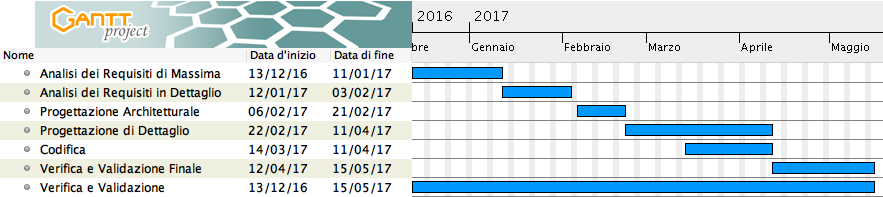
\includegraphics[scale=0.5]{Immagini/Gantt/TOT.png}
	\caption{Diagramma di Gantt, Monolith}
\end{figure}

\subsubsection{\ARM}
Periodo: dal 13/12/2016 all'11/01/2017. \\

L'inizio del periodo di \ARM\ corrisponde all'inizio del progetto. In questo periodo il gruppo deve scegliere un \termine{capitolato} e cominciare a lavorare con il fine ultimo di aggiudicarselo.\\
Ciò comporta la stesura dei seguenti documenti:
 \begin{itemize}
 \item Esterni:
 	\begin{itemize}
 	 \item \AdR
 	 \item \PdP
	 \item \PdQ
 	\end{itemize}
 \item  Interni:
	\begin{itemize}
	\item \SdF
	\item \NdP
	\end{itemize} 
 \end{itemize}
 Il carico di lavoro viene suddiviso principalmente tra i ruoli di \An, \Am, \Ver\ e \Pm.
 Il periodo termina con una milestone esterna, corrispondente alla consegna dei documenti per la \RR.
 
 \begin{figure}[H]
	\centering 
	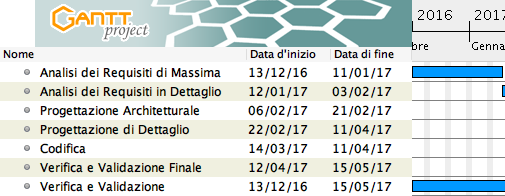
\includegraphics[scale=0.5]{Immagini/Gantt/ARM.png}
	\caption{Diagramma di Gantt, \ARM}
\end{figure}

\subsection{\ARD}
Periodo: dal 12/01/2017 al 03/02/2017 \\

Questo periodo inizia subito dopo la consegna dei documenti per la \RR. Il termine corrisponde ad una \termine{milestone} interna che coincide con l'inizio del periodo successivo, la \PA.\\
Il \termine{gruppo} in questo periodo si impegnerà ad identificare, ampliare e fissare definitivamente i requisiti richiesti per lo svolgimento del progetto.\\
Verranno inoltre effettuate le modifiche necessarie, rilevate in seguito all'esito della \RR\, nei vari documenti.\\
I ruoli coinvolti maggiormente in questo periodo sono: \An, \Am, \Pm\ e \Ver.

\begin{figure}[H]
	\centering 
	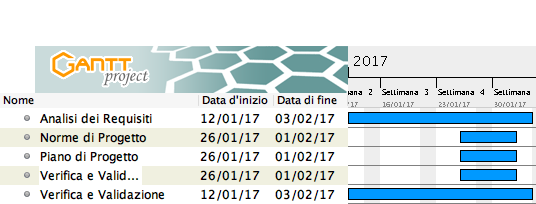
\includegraphics[scale=0.5]{Immagini/Gantt/ARD.png}
	\caption{Diagramma di Gantt, \ARD}
\end{figure}

\subsection{\PA}
Periodo: dal 06/02/2017 al 21/02/2017 \\

Inizia in seguito alla terminazione dell'\ARD\ ed il suo il termine prefissato coincide con una \termine{milestone} interna.
Il \termine{gruppo} si pone l'obbiettivo di eseguire e fissare definitivamente la progettazione del sistema ad alto livello e di redigere il documento \ST.\\
In quest'ultimo documento i \ProgP\ dovranno descrivere, ad alto livello, le scelte progettuali ed il \termine{design-pattern} scelti per la realizzazione dell'architettura generale del \termine{prodotto}. Vengono inoltre incrementati i documenti \NdP, \PdP, \PdQ\ e \Gl.\\
In questo periodo i ruoli maggiormente interessati sono: \Prog, \Pm, \Ver\ e \Am.

 \begin{figure}[H]
	\centering 
	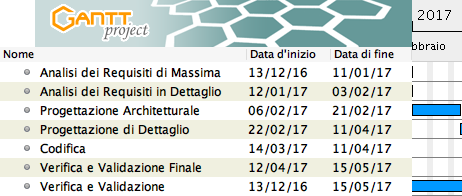
\includegraphics[scale=0.5]{Immagini/Gantt/PA.png}
	\caption{Diagramma di Gantt, \PA}
\end{figure}

\subsection{\PD}
Periodo: dal 22/02/2017 all'11/04/2017\\

Dal seguente periodo lo svolgimento dei passi successivi segue il \termine{Modello Incrementale}, ovvero verranno realizzati prima i requisiti essenziali, poi quelli desiderabili e infine quelli facoltativi per ridurre il rischio di fallimento. 
Inizia in seguito all'approvazione della \PA\ e si conclude entro la consegna del prodotto alla \RQ.
Il gruppo si impegna a terminare la \PD\ almeno delle funzionalità essenziali per il 06/03/2017, che coincide con una \termine{milestone} esterna per la consegna dei documenti della \RP.\\
Il gruppo, ad ogni incremento, si impegna ad intraprendere e completare le seguenti attività:
\begin{itemize}
\item
Redigere o aggiornare il documento \DDP\ in cui i \ProgrP\ e i \ProgP\ devono descrivere il comportamento e le interazioni tra i vari componenti del sistema, basandosi sul documento di \ST.
\item
Incrementare i documenti \NdP, \PdP, \PdQ\ e \Gl.
\end{itemize}
In questo periodo i ruoli maggiormente impegnati sono quelli di \Prog, \Progr, \Pm, \Ver\ e \Am.

 \begin{figure}[H]
	\centering 
	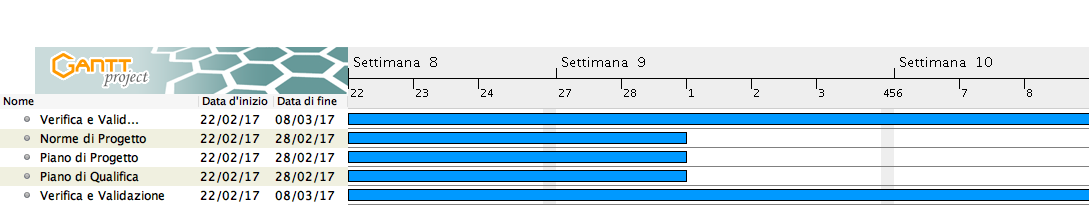
\includegraphics[scale=0.5]{Immagini/Gantt/PD.png}
	\caption{Diagramma di Gantt, \PD}
\end{figure}

\subsubsection{\COD}
Periodo: dal 14/03/2017 all'11/04/2017. \\

Il periodo di \COD\ avviene in concorrenza a quello di \PD ed inizia una volta completata la progettazione dettagliata delle funzionalità essenziali. Essa si conclude con la consegna del prodotto alla \RQ. L'obiettivo finale consiste nel consegnare un prodotto completo, e le attività che ad ogni incremento verranno eseguite a tal fine sono le seguenti:
\begin{itemize}
	\item \COD: I \ProgrP\ devono sviluppare il codice del prodotto software attenendosi il più possibile a quanto scritto dai \ProgP\ nel documento \DDP. L'attività di \COD\ deve essere fatta seguendo, iterativamente, i seguenti passi:
			\begin{itemize}
				\item \termine{Codifica} dell'incremento svolto dai \ProgP.
				\item \termine{Verifica} dell'incremento.
			\end{itemize}
	\item Stesura o ampliamento del \MU: questo documento è destinato all'utilizzatore finale del prodotto che, tramite esso, deve essere in grado di capire le principali funzionalità del sistema e come utilizzarle.
	\item \termine{Verifica} dei documenti, della progettazione e del software prodotto con gli strumenti definiti nelle \NdP.
\end{itemize}
I ruoli maggiormente interessati sono quelli di \Am, \Pm, \Prog, \Progr\ e \Ver.

 \begin{figure}[H]
	\centering 
	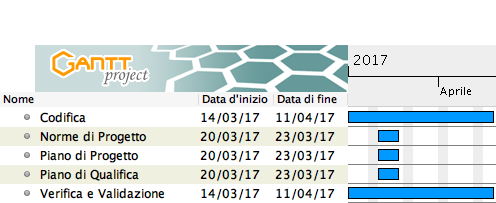
\includegraphics[scale=0.5]{Immagini/Gantt/COD.png}
	\caption{Diagramma di Gantt, \COD}
\end{figure}

\subsubsection{Verifica e Validazione}
Periodo: dal 16/12/2016 al 14/05/2017.\\

Questo periodo, come si può osservare dalla data di inizio, è trasversale a tutti i periodi. Infatti, per garantire ad ogni incremento efficacia ed efficienza del prodotto, le operazioni di \termine{testing}, \termine{verifica} e \termine{validazione} vengono eseguite durante tutto il corso del progetto.\\

\paragraph{\VV}
Periodo: dal 12/04/2017 al 15/05/2017 \\

Al termine della \PD e \COD\ verranno effettuati ed intensificati tutti i test necessari per garantire che il prodotto soddisfi tutti i requisiti dell'\AdR e la correzione di eventuali errori nel codice e/o nei vari documenti.
Le attività prevedono di:
\begin{itemize}
	\item Effettuare dei test di sistema.
	\item Incrementare, correggere o aggiornare i documenti di: \MU, \NdP, \PdP, \PdQ\ e \Gl.
	\item Verificare tutti i documenti sopra citati.
	\item Verificare il corretto funzionamento del prodotto correggendo eventuali errori.
\end{itemize}
In questo periodo i ruoli maggiormente interessati sono quelli di \Ver, \Prog, \Am\ e \Pm.

 \begin{figure}[H]
	\centering 
	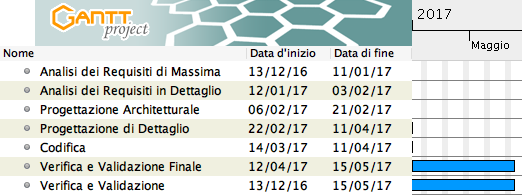
\includegraphics[scale=0.5]{Immagini/Gantt/VV.png}
	\caption{Diagramma di Gantt, \VV}
\end{figure}